\documentclass[8pt]{beamer} 
%\usepackage{pgf}
\usepackage{animate}
\usepackage{graphicx}
\usepackage{subfigure}

\usepackage[utf8]{inputenc}
\usepackage[T1]{fontenc}
\usepackage{lmodern}

\usepackage{amssymb,amsmath,amscd,amsfonts,amsthm,bbm,bm}
\usepackage{wasysym}
%\usepackage{graphicx}
%\usepackage{animate}
%\usepackage{psfrag}
%\usepackage{paralist}
\usepackage{color}
%\usepackage{float}
%\usepackage{relsize}
%\usepackage{euscript}
%\usepackage{setspace}
%\usepackage{flushend}
%%\usepackage[usenames,dvipsnames]{xcolor}
\usepackage{tikz}

\usepackage{pgfplots}
\usetikzlibrary{arrows,shapes,decorations,backgrounds}
\usepackage{tkz-berge}
\DeclareMathOperator*{\argmin}{argmin}
\DeclareMathOperator*{\argmax}{argmax}
\newcommand{\SNR}{\mathsf{SNR}}
\newcommand{\Q}{\mathbb{Q}}
% *** TPT STYLE ***

\setbeamerfont{subsection in toc}{size=\large}

\definecolor{colorframetitle}{RGB}{191,18,56} % Title of frames
\definecolor{redbox}{RGB}{191,18,56} % 
\definecolor{blackbox}{RGB}{0,0,0} % 
\definecolor{brownbox}{RGB}{128,99,90} % 

\usepackage[absolute,overlay]{textpos}
\usepackage{listings}
\usepackage{hyperref}

\setlength{\TPHorizModule}{1mm}
\setlength{\TPVertModule}{1mm}

\usepackage{tikz}
\usetikzlibrary{decorations.pathreplacing,calc}
\usetikzlibrary{arrows,shapes,snakes,automata,backgrounds,petri}
\usepackage{scalefnt}



\newcommand{\tikzmark}[1]{\tikz[overlay,remember picture] \node (#1) {};}

\tikzstyle{mybox} = [draw=redbox, fill=redbox!20, very thick,
    rectangle, rounded corners, inner sep=10pt, inner ysep=20pt]
\tikzstyle{fancytitle} =[fill=redbox, text=white, rectangle]


\newcommand{\MyLogo}{
%\begin{textblock}{14}(117.2,0.7)
\begin{textblock}{14}(108.8,86)

\includegraphics[width=0.8cm]{figures/tpt}

\includegraphics[width=1.1cm]{figures/cisco.png}
 \end{textblock}
}


%\begin{textblock}{14}(117.2,0.7)








\usepackage{beamerthemesplit}

\setbeamercolor{itemize item}{fg=redbox}
\setbeamercolor{structure}{fg=redbox, bg=red}
\setbeamercolor{block title}{bg=brownbox,fg=white}
\setbeamercolor{block title alerted}{bg=redbox,fg=white}
\setbeamercolor{block body alerted}{bg=brownbox!0,fg=black}
\setbeamercolor{block title example}{bg=black, fg=white}
\setbeamercolor{palette primary}{fg=black,bg=white} % changed this
\setbeamercolor{palette secondary}{use=structure,fg=structure.fg!100!white} % changed this
\setbeamercolor{palette tertiary}{use=structure,fg=structure.fg!100!white} % changed this
\setbeamercolor*{palette quaternary}{fg=black,bg=white} % outline on top left
\setbeamercolor{background canvas}{bg=white, fg=black} 
\setbeamercolor{frametitle}{fg=colorframetitle}


% First  frame
\newcommand{\RectanglesOfMainSlide}{%
\raisebox{0mm}[0pt][0pt]{%
\begin{pgfpicture}{0mm}{0mm}{0mm}{0mm}
\pgfsetlinewidth{5mm}
\color{redbox}
\pgfline{\pgfpoint{-4mm}{-12mm}}{\pgfpoint{24mm}{-12mm}}
\color{blackbox}
\pgfline{\pgfpoint{24mm}{-12mm}}{\pgfpoint{52mm}{-12mm}}
\color{brownbox}
\pgfline{\pgfpoint{52mm}{-12mm}}{\pgfpoint{80mm}{-12mm}}
\end{pgfpicture}}}

\newcommand{\makeFirstFrame}{
\setbeamertemplate{footline}{} 
\frame[plain]{
\begin{columns}[c]
\column{3cm}
\vspace{-2cm}\\

\includegraphics[width=1.5cm]{figures/tpt}

\includegraphics[width=2.2cm]{figures/cisco.png}\\
\column{7cm}
\vspace{1cm}\\
\LARGE{\textbf{\theTitle}}\\
\vspace{0.5cm}
\normalsize{\theAuthors}\\
\vspace{0.5cm}
\normalsize{\theResponsible}\\
\vspace{0.5cm}

\normalsize{\theConferenceAndPlace}\\
\vspace{-1cm}
\RectanglesOfMainSlide
\end{columns}
}
\activateFootline
}


% Frames decoration

\newcommand{\RectanglesBeforeTitle}{%
\raisebox{0mm}[0pt][0pt]{%
\begin{pgfpicture}{0mm}{0mm}{0mm}{0mm}
\pgfsetlinewidth{5mm}
\color{redbox}
\pgfline{\pgfpoint{-2mm}{2.2mm}}{\pgfpoint{4mm}{2.2mm}}
\color{blackbox}
\pgfline{\pgfpoint{4mm}{2.2mm}}{\pgfpoint{10mm}{2.2mm}}
\color{brownbox}
\pgfline{\pgfpoint{10mm}{2.2mm}}{\pgfpoint{16mm}{2.2mm}}
\end{pgfpicture}}}

\setbeamertemplate{frametitle}{
\begin{columns}[t]
\column{16mm}
\RectanglesBeforeTitle 
\column{10.7cm}
\strut\textbf{\insertframetitle}\strut
\end{columns}
}

% Foot line

\newcommand{\Ffootline}{
\MyLogo
\begin{tikzpicture}
 \fill [color=white, fill=redbox] (-1, -0.05) rectangle (1, 0.30);
\node[white, right] (note1) at (-1, 0.10) {\insertframenumber/\inserttotalframenumber};
\node[white, left] (note1bis) at (0.98, 0.10) {\theDate};
 \fill [color=white, fill=blackbox] (1.05, -0.05) rectangle (4.5, 0.30);
\node[white, align=center] (note2) at (2.27, 0.12) {Institut Mines-Telecom};
 \fill [color=red, fill=brownbox] (3.55, -0.05) rectangle (9.75, 0.30);
\node[white, align = center] (note3) at (6.65, 0.10) {\thefootnotedef};

%\node[white] (note3) at (7.5, 0.10) {\theTitle};
\end{tikzpicture}
}

\newcommand{\activateFootline}{
\setbeamertemplate{footline}{
\usebeamerfont{structure}
\Ffootline
}
}


% *** END OF TPT STYLE ***


%remove navigation symbols
\setbeamertemplate{navigation symbols}{}

% To show the outline at the beginning of each section
\AtBeginSection[]{
   \begin{frame}
   \frametitle{Plan}
   %\begin{center}{\LARGE Outline }\end{center}
   \tableofcontents[currentsection,hideothersubsections]
   \end{frame} 
}

\newcommand{\mytilde}{\raise.17ex\hbox{$\scriptstyle\mathtt{\sim}$}}

\newcommand{\tikzgrid}{
\begin{pgfonlayer}{background}
\draw[gray!50]
(current bounding box.south west)
grid[step=.2] (current bounding box.north east);
\draw[red!50]
(current bounding box.south west)
grid (current bounding box.north east);
\end{pgfonlayer}
}

\newcommand*{\ExtractCoordinate}[3]{\path (#1); \pgfgetlastxy{#2}{#3};}%

\newdimen\tlx
\newdimen\tlx
\newdimen\brx
\newdimen\bry

%% To FILL to customize presentation with the TPT style

\newcommand{\theTitle}{Routing Algorithms in NDN Networks}
\newcommand{\thefootnotedef}{Routing Algorithms in NDN networks}
\newcommand{\theAuthors}{shahab SHARIAT BAGHERI}
\newcommand{\theResponsible}{Luca MUSCARIELLO\\Beatrice PESQUET \\ Pablo PIANTANIDA}
\newcommand{\theConferenceAndPlace}{Internship Defense \\
Salle F801, TELECOM ParisTech}
\newcommand{\theDate}{9/26/2016}

%%%%%%

\DeclareMathOperator{\tr}{Tr}
\DeclareMathOperator{\support}{supp}
\DeclareMathOperator{\rank}{rank}
\DeclareMathOperator{\diag}{diag}
\newcommand{\bs}{\boldsymbol}

% Convergences 
\newcommand{\toaslong}{\xrightarrow[T\to\infty]{\text{p.s.}}}
\newcommand{\toasshort}{\xrightarrow{\text{p.s.}}}
\newcommand{\toprobalong}{\xrightarrow[T\to\infty]{{\cal P}}}
\newcommand{\toprobashort}{\xrightarrow{{\mathcal P}}}
\newcommand{\tolawlong}{\xrightarrow[T\to\infty]{{\cal L}}}
\newcommand{\tolawshort}{\xrightarrow{{\mathcal L}}}
\newcommand{\tolong}{\xrightarrow[T\to\infty]{}}
\newcommand{\norme}[1]{\left\Vert #1\right\Vert}

% Notations bb 
\newcommand{\N}{\mathbb N}
\newcommand{\R}{\mathbb R}
\newcommand{\Z}{\mathbb Z}
\newcommand{\C}{\mathbb{C}}
\newcommand{\E}{\mathbb{E}}
\newcommand{\1}{\mathbbm 1}
\newcommand{\PP}{\mathbb{P}}
 
\newcommand{\bl}{\{} 
\newcommand{\br}{\}} 

\def\bx{{\bf x}}\def\bx{{\bf x}}

\def\bA{{\bf A}}
\def\bY{{\bf Y}}
\def\bV{{\bf V}}
\def\bQ{{\bf Q}}
\def\ba{{\bf a}}
\def\bc{{\bf c}}
\def\bd{{\bf d}}
\def\bm{{\bf m}}
\def\bg{{\bf g}}
\def\bp{{\bf p}}
\def\bv{{\bf v}}
\def\bx{{\bf x}}
\def\by{{\bf y}}
\def\brho{{\boldsymbol \rho}}
\def\bDelta{{\boldsymbol \Delta}}
\def\bdelta{{\boldsymbol \delta}}

\def\bOmega{{\bf \Omega}}
\def\bbT{{\bf \mathbb{T}}}

\newtheorem{assumption}{Assumption}

\newcommand{\semitransp}[2][35]{\color{fg!#1}#2}

\begin{document}
 

 
\makeFirstFrame

\frame{
  \frametitle{Plan}
  \tableofcontents
}

\setbeamertemplate{blocks}[rounded][shadow=true]
\section{Internship Environment}

%%%%%%%%%%%%%%%%%%%%%%%%%%%%%%%
\subsection{CISCO \& PIRL}

\begin{frame}{CISCO \& PIRL}

Cisco Systems France.

\begin{center}
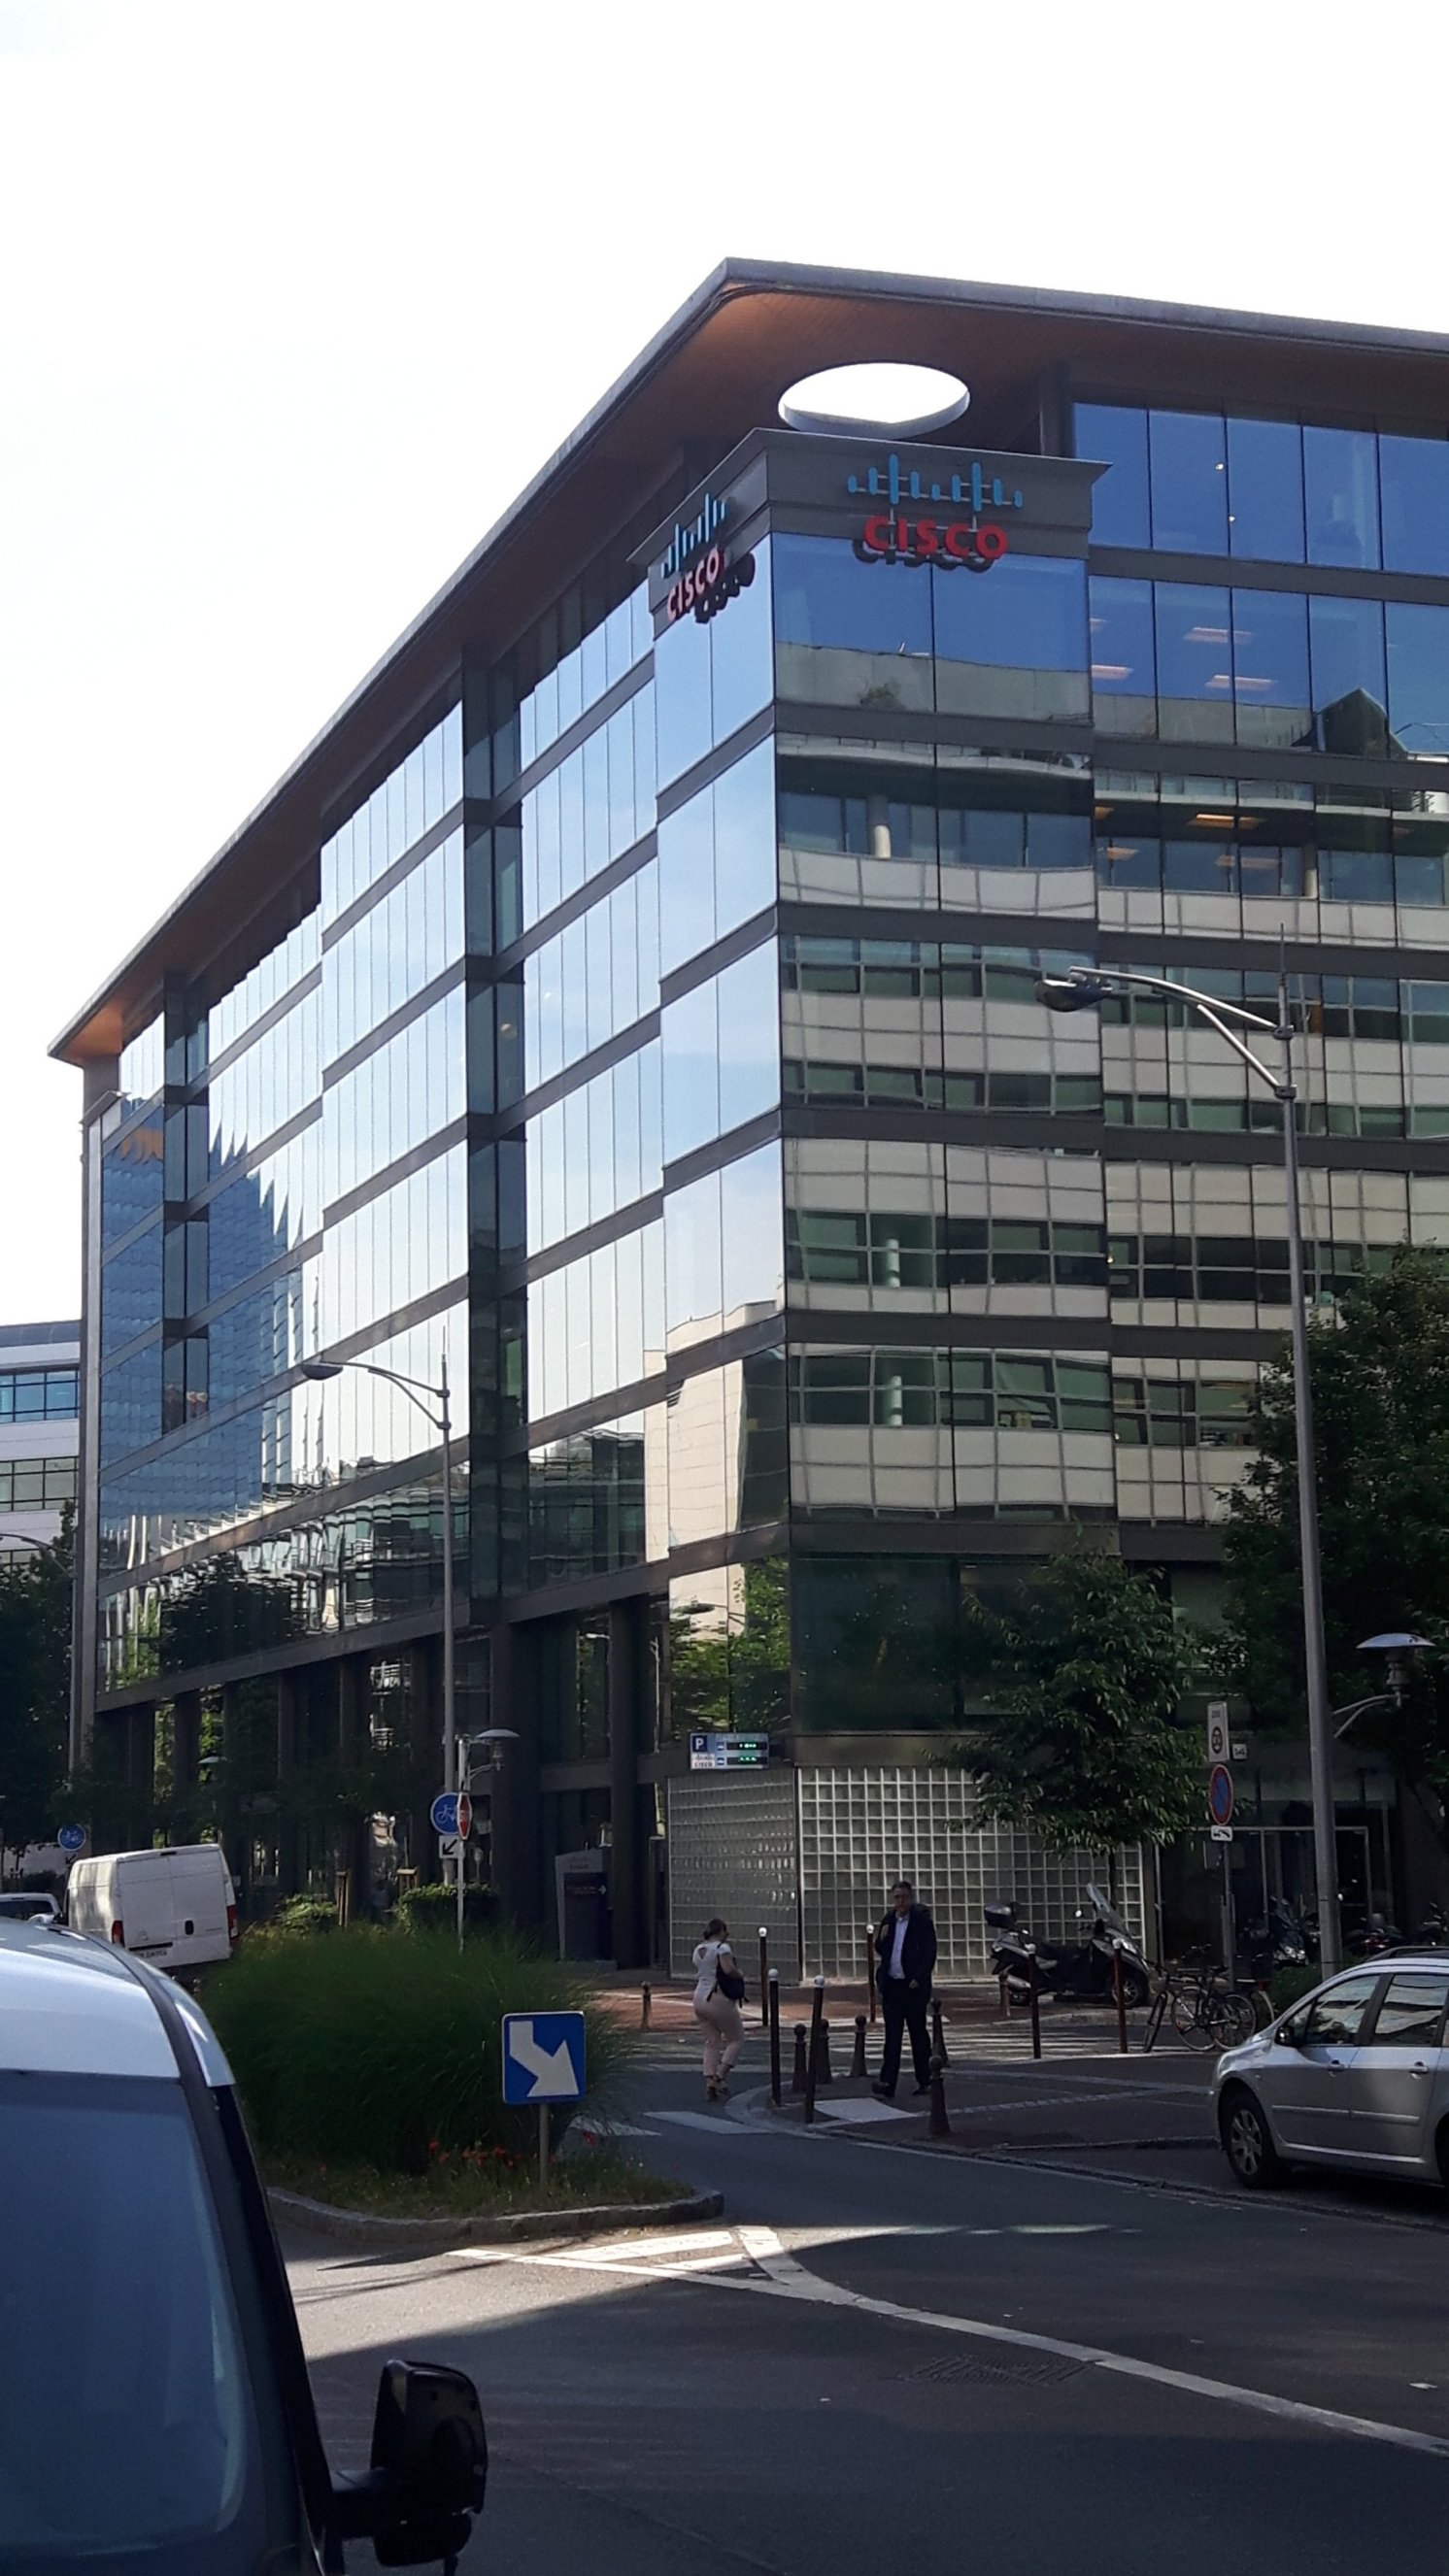
\includegraphics[scale=0.07]{figures/cisco.jpg}
\end{center}


\end{frame}
%
%\begin{frame}{PIRL}
%
%\textbf{P}aris \textbf{I}nnovation and and \textbf{R}esearch \textbf{L}aboratory.
%
%\end{frame}




%%%%%%%%%%%%%%%%%%%%%%%%%%%%%%%

\subsection{Goals and objectives}
\begin{frame}{Goals and objectives}

\only<1>{
Net Revenu for Video Delivery Applications

\begin{center}
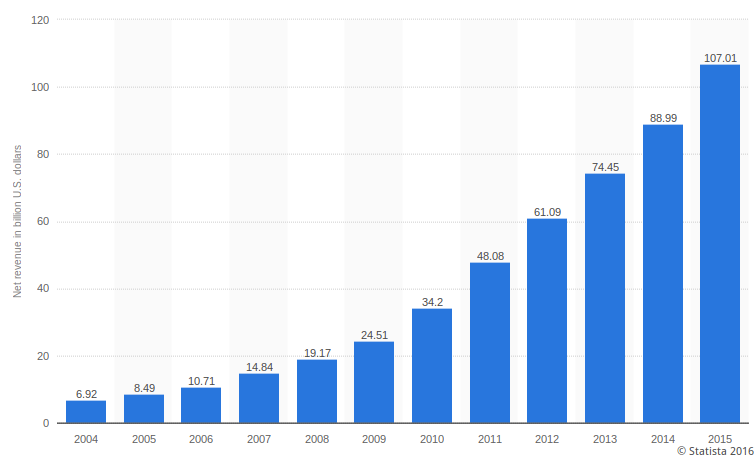
\includegraphics[scale=0.28]{figures/amazon.png}
\end{center}
}

\only<2>{
In 2016, More than 96 \% of internet traffic is content.

Video $\longrightarrow$ 60\%

File sharing $\longrightarrow$ 20\%

Web $\longrightarrow$ 20\%

\begin{center}
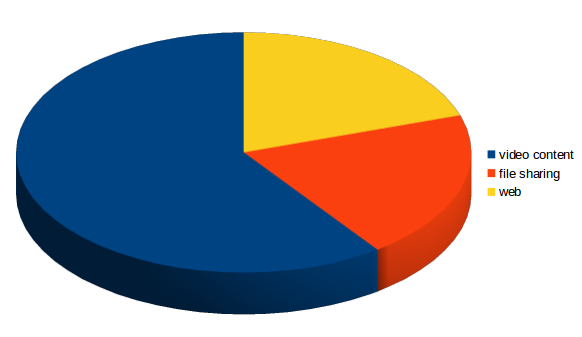
\includegraphics[scale=0.28]{figures/stat.png}
\end{center}

}

\only<3>{
Mobile vs PC Internet Traffic user $\longrightarrow$ 5G mobile networks


\begin{center}
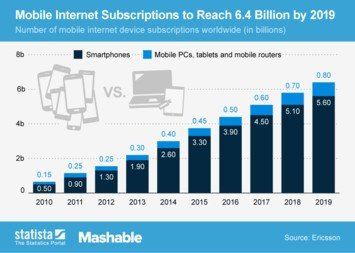
\includegraphics[scale=0.48]{figures/mobile.jpg}
\end{center}

}




\end{frame}

%%%%%%%%%%%%%%%%%%%%%%

%\subsection{Interference Alignment Techniques}
%\begin{frame}
%\frametitle{Interference Alignment Techniques}
%\vspace{-0.65cm}
%\uncover<1->{
%  \begin{block}{Which techniques to be used for IA ?}
%  \centering
%  \begin{itemize}
%  \item Linear Lattice-based Interference Alignment. 
%  \item The Compute-and-Forward (CoF) method described by [Nazer and Gastpar 2008].
%  \end{itemize}
%\end{block}}
%\vspace{-0.31cm}
%\uncover<2->{\begin{block}{Recent Research Studies ...}
%   \begin{itemize}
%   \item A coding scheme presented by [Khaleghi and Belfiore 2014] to improve the fading behavior of achievable sum rates defined in [Ordentlich \textit{et al.} 2012].
%   \item Lattice codes over Eisenstein integers presented for CoF [Tunali \textit{et al.} 2012] to achieve higher rates.
%   \end{itemize}}
%   \vspace{-0.15cm}
%   \uncover<3->{
%  For the \underline{complex-valued interference channels} need to realize more research.}
%  \vspace{0.1cm}
%  \uncover<4->{\\$\rightarrow$ In this research we focus on \textcolor{red}{\textit{the complex-valued interference channels}} and employing $\Z[i]$-lattice codes.
%   \end{block}}
%   \vspace{-0.31cm}
% \uncover<5->{
%   \begin{block}{In Compute-and-Forward scheme [Receiver's Point of View]}
%    \centering
%    \begin{enumerate}
%     \item Receiving linear combination of the transmitted codewords.
%     \item Deciding which equation(s) to be decoded.}
%     \uncover<6->{
%     \item Applying the corresponding Minimum Mean Square Error estimation (MMSE).
%     \item Decoding the equation(s) in $\Lambda_{\textrm{lattice}}$.
%    \end{enumerate}
%   \end{block}}
%\end{frame}

%%%%%%%%%%%%%%%%%%%%%%%
\section{Ideas and Strategies}

\subsection{ICN Brief Introduction}

\begin{frame}{Named Data networking (NDN)}
\only<1>{
\begin{itemize}
\item \textbf{N}amed \textbf{D}ata \textbf{N}etworking $\Rightarrow$ \textit{\textbf{Name}} base Philosophy vs TCP/IP \textit{\textbf{Calling}} Networking.

\item V.Jacobson et al proposition, \textit{Networking Named Content} 2009.

\item A Good fit network desiging for Video Delivery Applications in \textbf{5G}.

\end{itemize}

\begin{center}
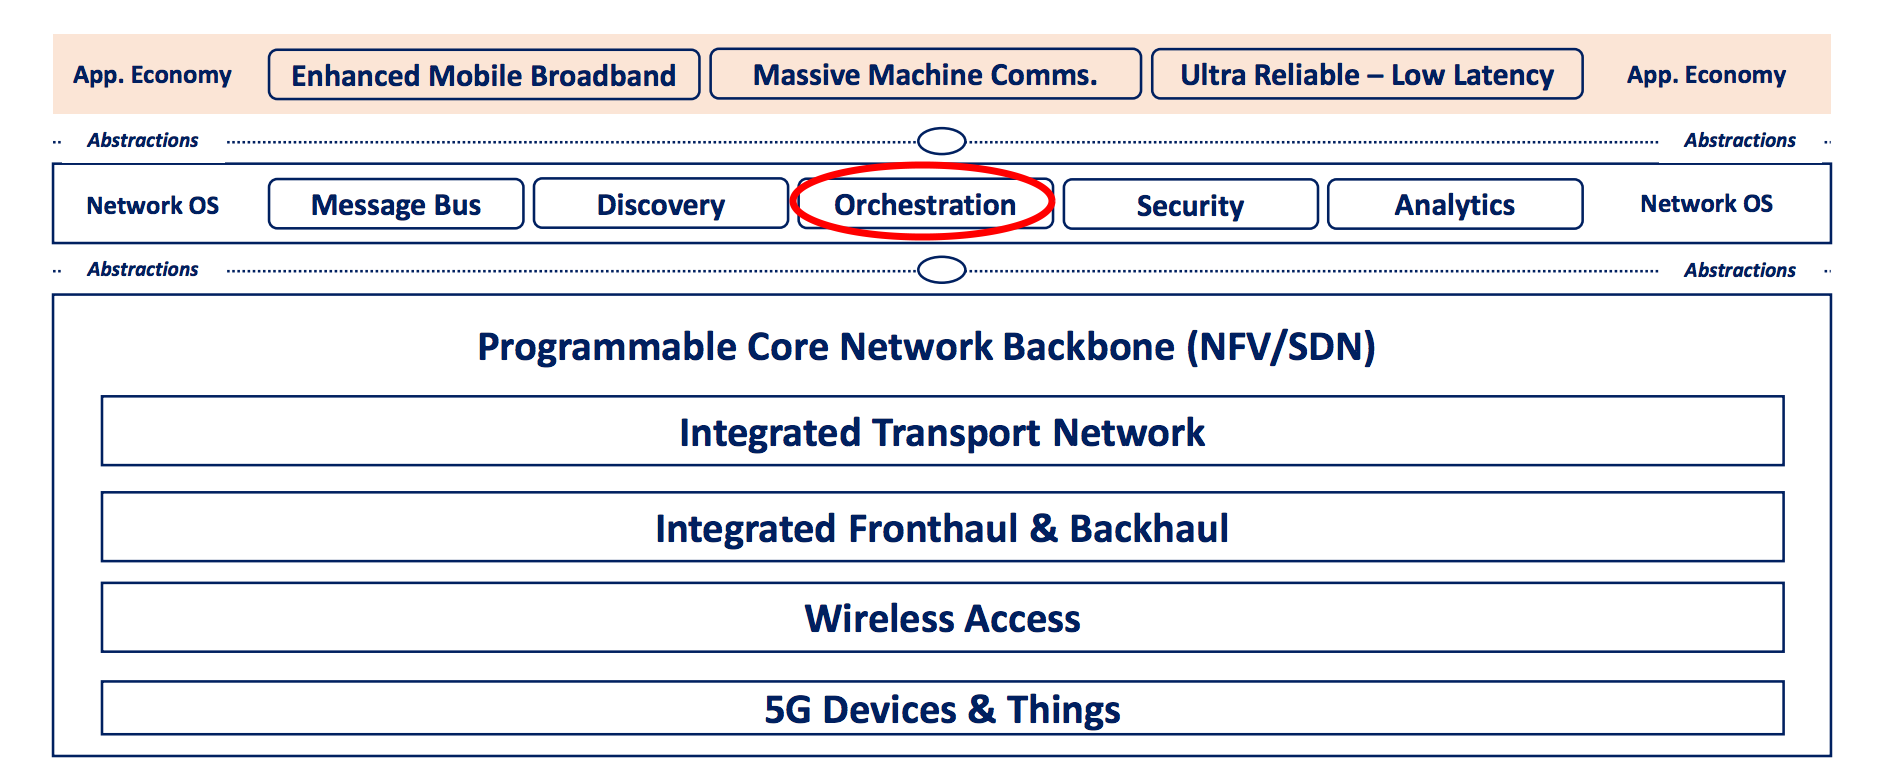
\includegraphics[scale=0.15]{figures/architecture.png}
\end{center}
}

\only<2>{
\begin{itemize}
\item \textbf{Lurch} is an orchestrator originally developped for ccnx. 
\item We developped Lurch:

\begin{itemize}
\item For NFD (NDN forwarder).
\item New Routing Strategies.
\item Different interfaces to interact with strategies at run time (Client, Repositories, forwading strategies, ...)

\begin{center}
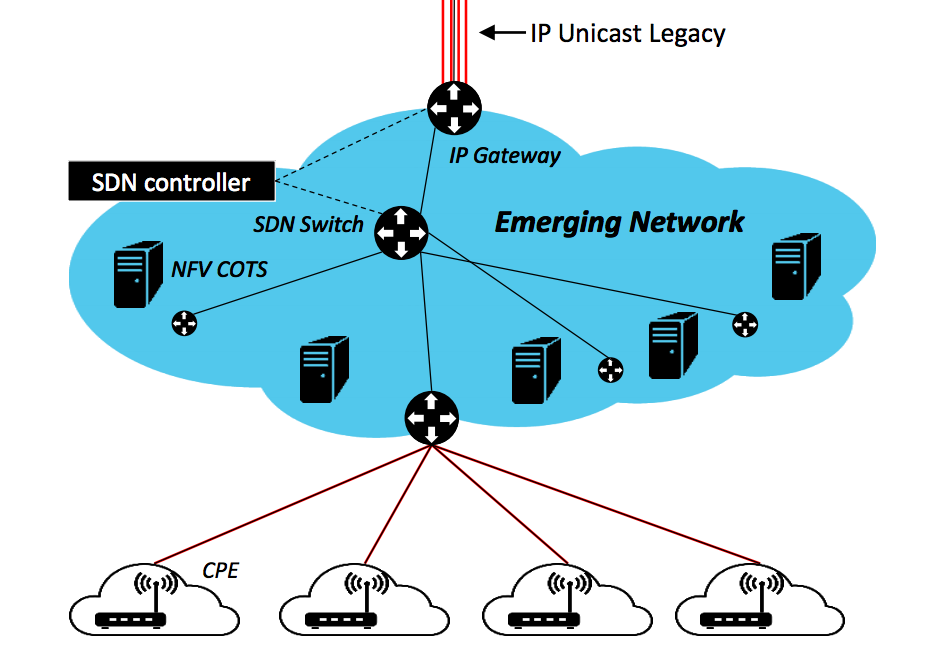
\includegraphics[scale=0.28]{figures/sdn.png}
\end{center}



\end{itemize}
\end{itemize} 
}

\only<3>{
\begin{center}
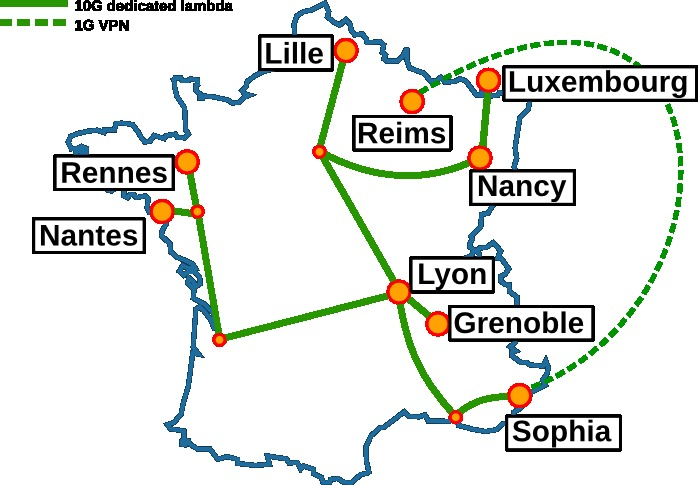
\includegraphics[scale=0.48]{figures/grid.jpg}
\end{center}
}



\end{frame}





\subsection{Virtualization and Linux Containers}

\subsubsection{Virtualization and Linux Containers}

\begin{frame}{Virtualization and Linux Containers}
\only<1>{
Virtual Machines (VM) vs Linux Containers.

\begin{center}
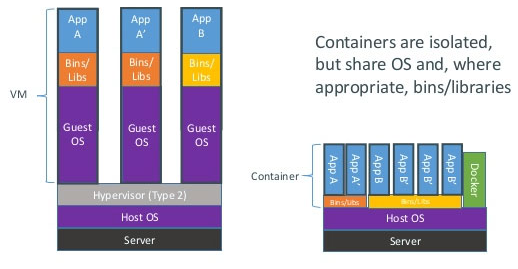
\includegraphics[scale=0.42]{figures/lxc.png} 
\end{center}

}

\end{frame}

%%%%%%%%%%%%%%%%%%%%%
\subsubsection{Routing Strategies}
\begin{frame}{Routing Strategies}
We proposed 4 different routing strategies for different situation of networks which can cover all of needs:
\begin{itemize}

\item \textbf{TreeOnConsumer} : N clients searching the same content from one repository detected by Lurch (Multicast mode).

\item \textbf{TreeOnProducer}: One client who gets the packet from N Repositories of needed data.

\item \textbf{MinCostMultiPath}: Using different paths with Equal Cost to retrieve the data using a proper forwarder strategy (load-balancing).

\item \textbf{MaxFlow}: Allow to maximize the throughput using paths based on maximum flow algorithm between clients and repositories.

\end{itemize}
\end{frame}
%%%%%%%%%%%%%%%%%%%%%%%%

\section{Routing Algorithms Results}

\subsection{TreeOnConsumer}

\begin{frame}{TreeOnConsumer}

\only<1>{
One producer to multiple consumer.

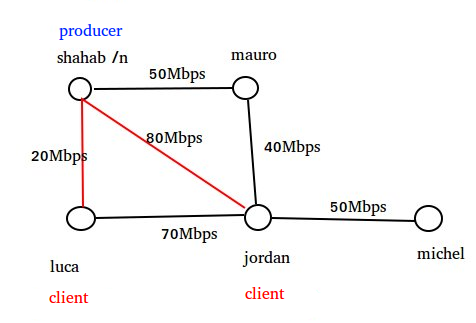
\includegraphics[scale=0.32]{figures/TreeOnConsumer.png} 
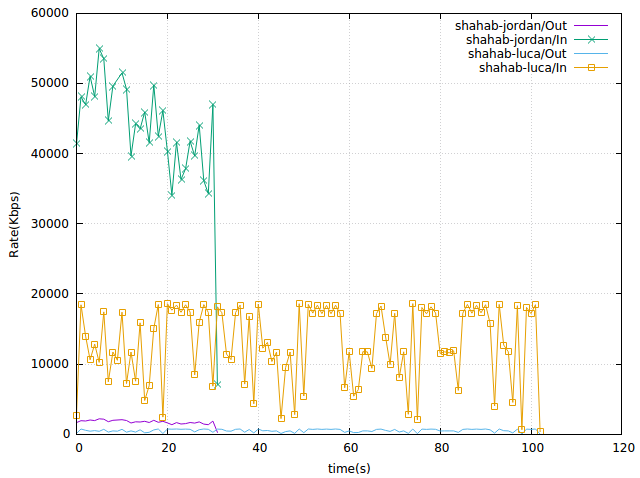
\includegraphics[scale=0.22]{figures/treeonconsumer.png} 
}
\only<2>{
One producer to multiple consumer.

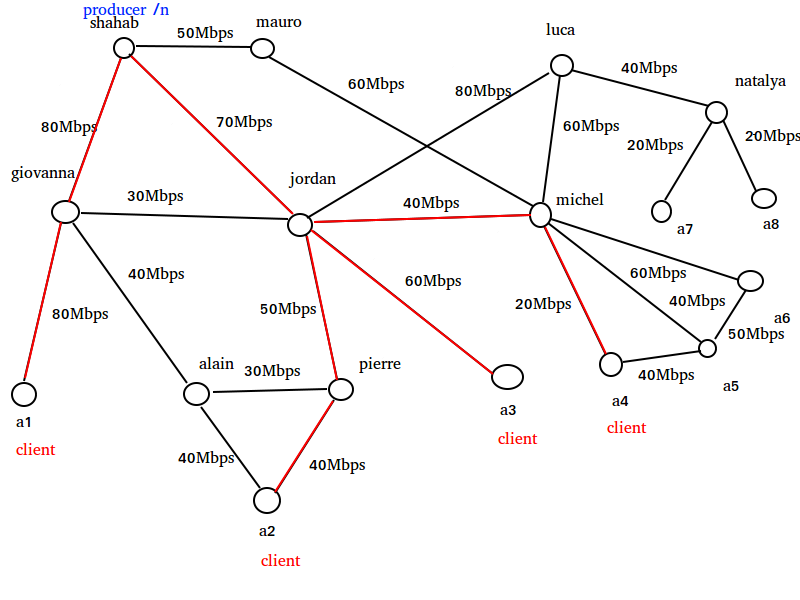
\includegraphics[scale=0.22]{figures/TreeOnConsumer_big.png} 
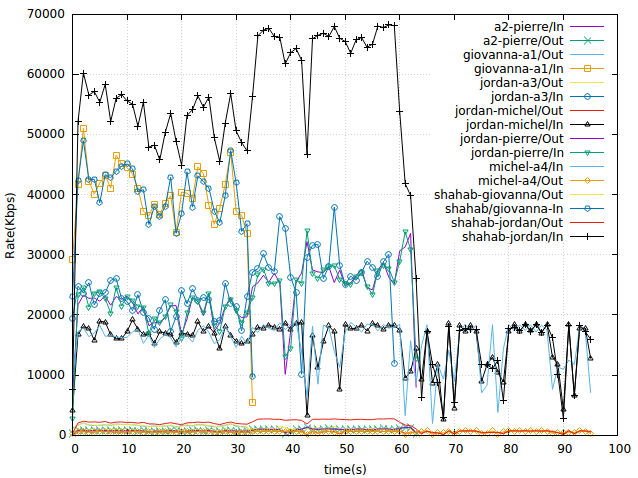
\includegraphics[scale=0.23]{figures/treeonconsumer_big.png} 

}

\end{frame}

%%%%%%%%%%%%%%%
\subsection{TreeOnProducer}

\begin{frame}{TreeOnProducer}
\only<1>{
One Consumer to multiple producer.

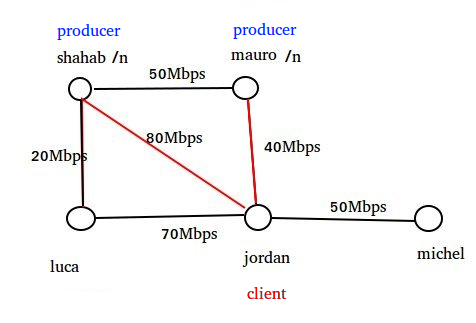
\includegraphics[scale=0.32]{figures/TreeOnProducer.png} 
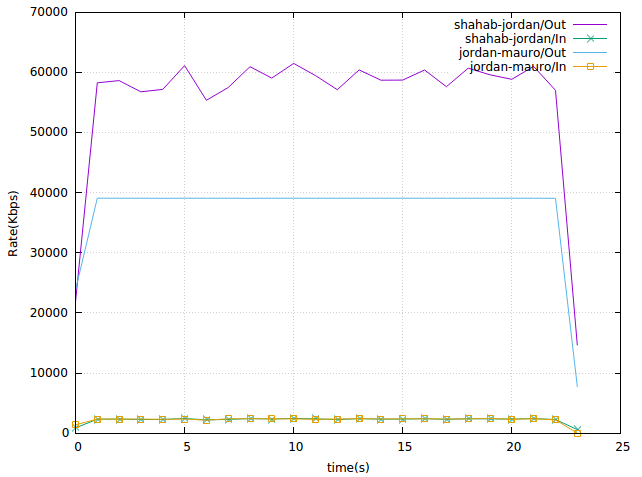
\includegraphics[scale=0.22]{figures/treeonproducer.png} 
}
\only<2>{
One Consumer to multiple producer.

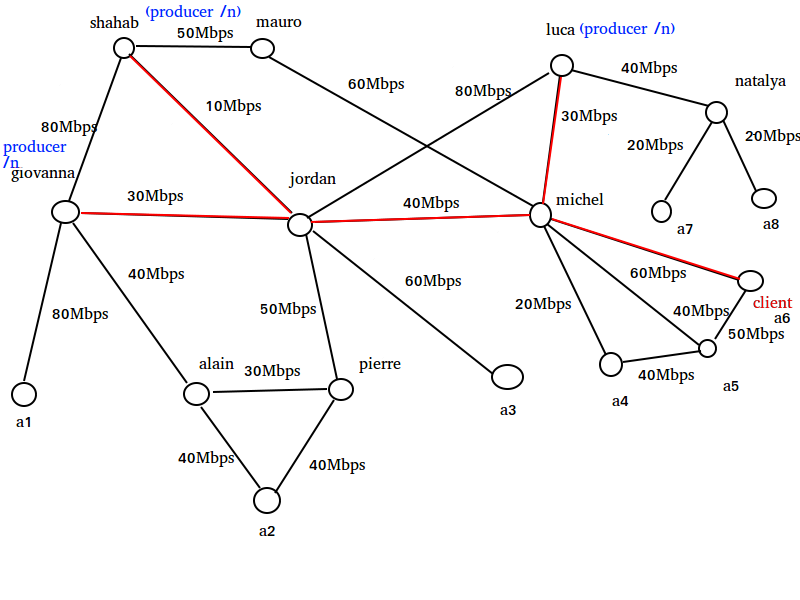
\includegraphics[scale=0.22]{figures/TreeOnProducer_big.png} 
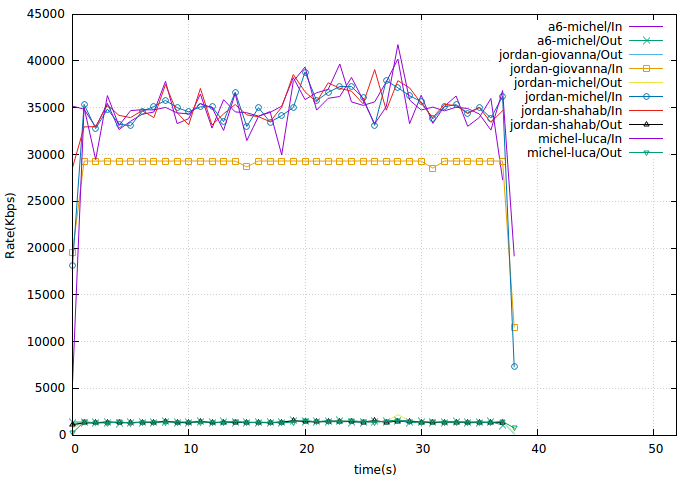
\includegraphics[scale=0.21]{figures/treeonproducer_big.png} 

}



\end{frame}


\subsection{MinCostMultiPath}

\begin{frame}{MinCostMultiPath}


\only<1>{
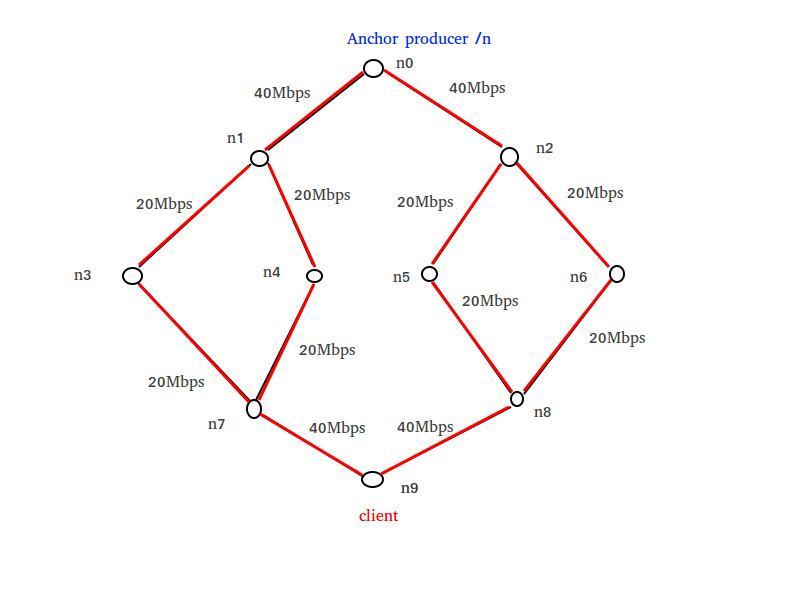
\includegraphics[scale=0.22]{figures/Load.png} 
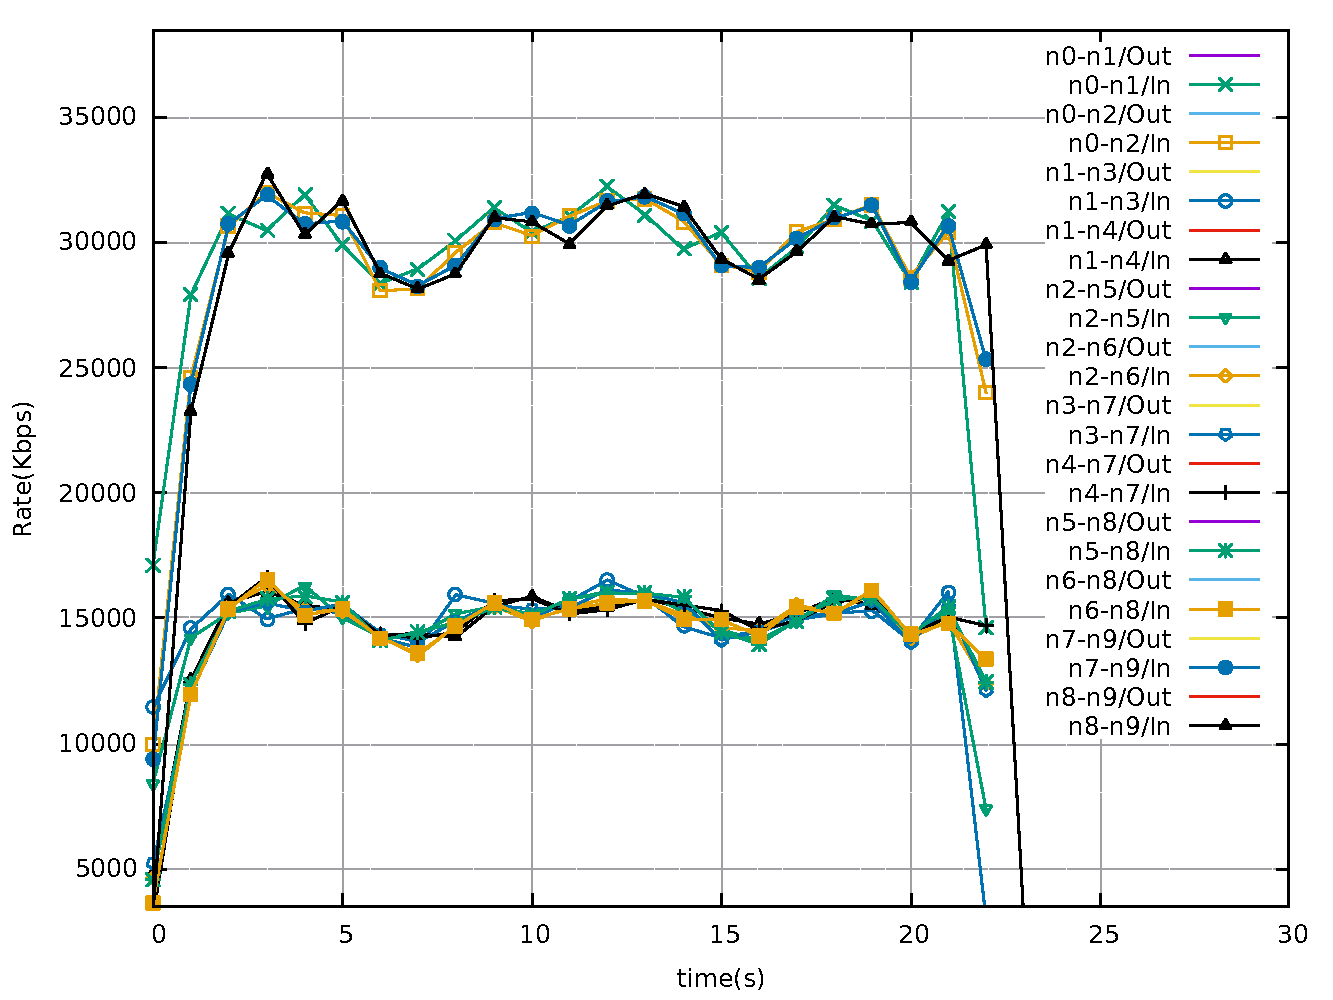
\includegraphics[scale=0.25]{figures/load.pdf} 
}
\only<2>{
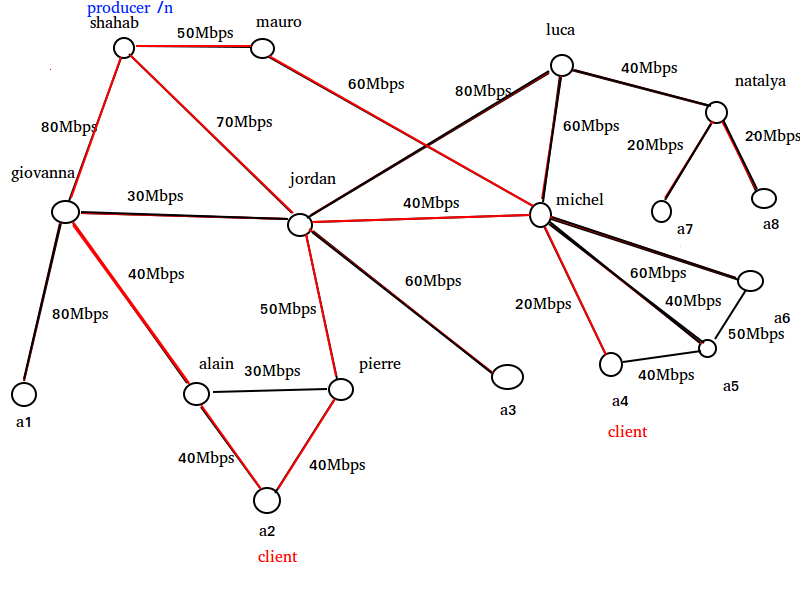
\includegraphics[scale=0.22]{figures/MinCostMultipath_big.png} 
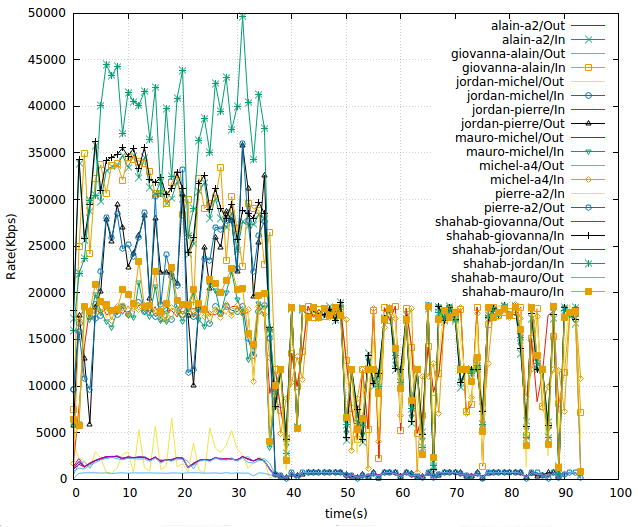
\includegraphics[scale=0.21]{figures/mincostmultipath_big.png} 

}


\only<3>{

Producer Mobility with Routing update.

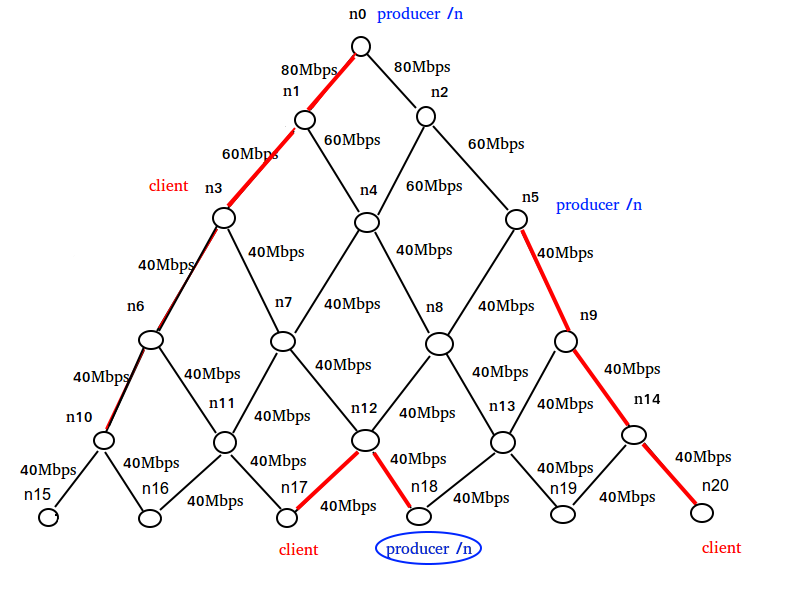
\includegraphics[scale=0.20]{figures/Step1.png} 
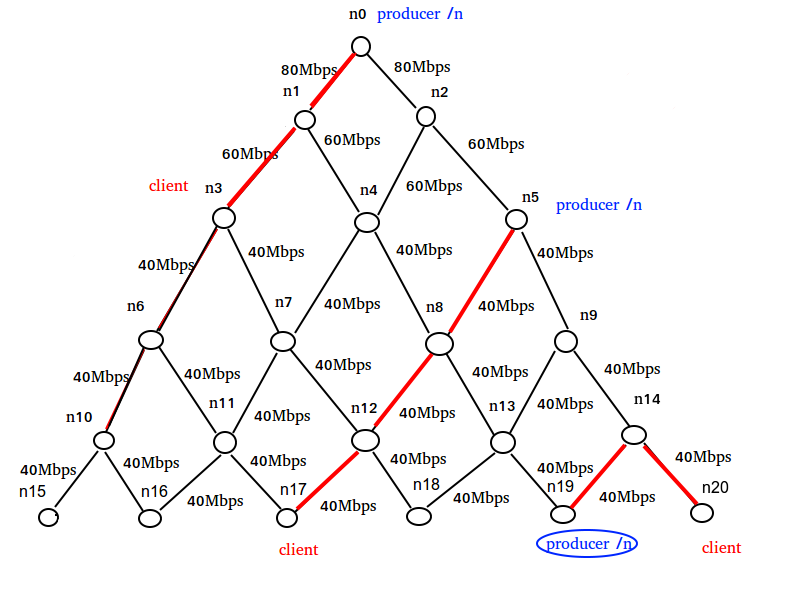
\includegraphics[scale=0.20]{figures/Step2.png} 


}



\end{frame}




\subsection{Maximum Flow}

\begin{frame}{Maximum Flow}


\only<1>{
Maximum Flow algorithm chooses the path which maximizes through from consumer to producer.

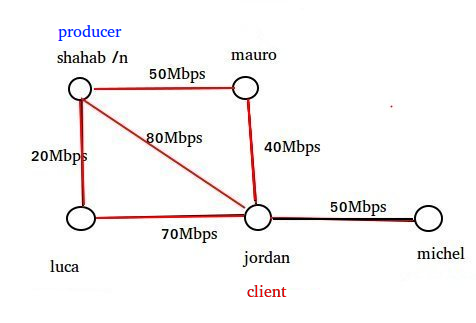
\includegraphics[scale=0.32]{figures/MaxFlow.png} 
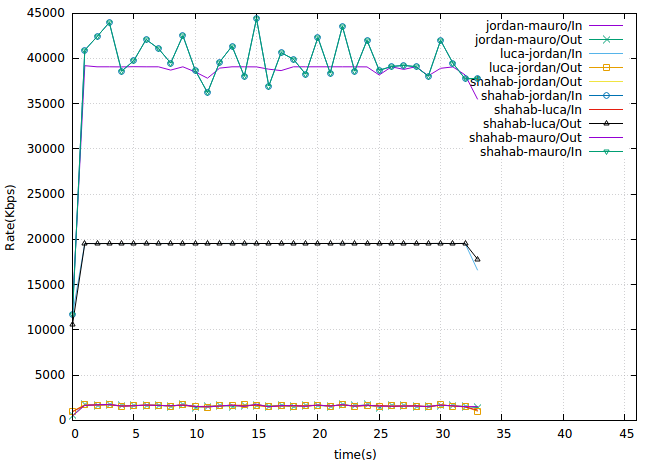
\includegraphics[scale=0.22]{figures/maxflow.png} 
}
\only<2>{
Maximum Flow algorithm chooses the path which maximizes through from consumer to producer.

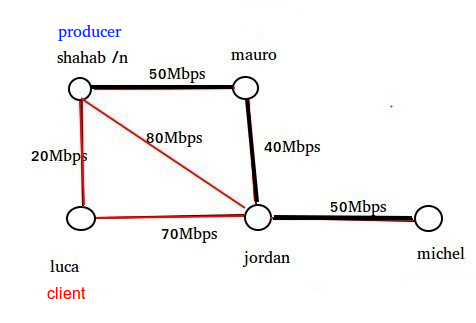
\includegraphics[scale=0.42]{figures/MaxFlow2.png} 


}




\end{frame}

\section{Conclusion}

\begin{frame}{Conclusion}
\begin{itemize}
 
\item There is always some limitations in practical against pure theoritical works which can be seen when you work experimental..  
\item ICN is one of the most challenging domain who has a lot of passion in research and development.
\item Software Define Networking is beautiful idea which allows to interact with your network on data centers and to shift heavy calculations.

\item Coding is one of way that you can realize your system.
\end{itemize}

\end{frame}

%%%%%%%%%%%%%%%%%%%%%%%

\begin{frame}



\begin{figure}[h!]
  \centering
    
\includegraphics[scale=0.5]{figures/merci.jpg}
\end{figure}



\end{frame}



\end{document}
